% !TeX encoding = ISO-8859-1
%%%%%%%%%%%%%%%%%%%%%%%%%%%%%%%%%%%%%%%%%%%%%%%%%%%%%%%%%%%%
\chapter{Theoretical Framework}
\label{ch:thefram}
This chapter presents a theoretical definition of all the main concepts used in the implementation of a traffic scene understanding system.

The section ~\ref{sec:cnn} covers the theoretical principles of Convolutional Neural Network and how they yield a semantic labeling process. Applications not related to computer vision tasks are beyond the scope of this thesis and omitted.

Section ~\ref{sec:secseg} explains several segmentation methods used in the temporary consistent segmentation. Efficient graph-based segmentation from \textcite{felzenszwalb2004efficient} and Watershed cuts as described in \textcite{cousty2009watershed}. These segmentation methods are characterized for requiring a small computationally effort and being fast enough to allow their use in real-time applications.  

To end this chapter, section ~\ref{sec:tempconsseg} describes how causal segmentation is yield (e.g. previous frames matching, Optical Flow and combined used with frame-by-frame approach). 
%In order to clarify how the traffic scene understanding is done via semantic segmentantion, Convolutional Neural Networks (CNNs), Efficient Graph-based segmentation, Optical flow and Causal Segmentation are explained in detail in the subsequent sections. 
%In this Chapter the basics of Convolutional Neural Networks are first presented for a better understanding of the chosen semantic segmentation approach. Explanation of how Neural Networks were modified in order to handle vision tasks. The uses of Convolutional Neural Networks will often focus on this work needs. Some other applications for Convolutional Neural Networks are beyond the scope of this thesis. \textcite{szegedy2014going} 

\section{Convolutional Neural Networks}
\label{sec:cnn}

Convolutional Neural Networks (CNNs) are Neural Networks which perform a \textbf{convolution instead of a matrix multiplication in at least one of their layers} (\textcite{Bengio-et-al-2015-Book}). In order to process data inside a CNN, this must have a grid-like topology. CNNs are loosely based on neuroscientific principles and inspired on the mammalian vision system.

CNNs were firstly introduced in \textcite{fukushima1980neocognitron}, but it was until \textcite{le1990handwritten} (introduction of backpropagation) and \textcite{lecun1998gradient} where they were successfully implemented to solve visual tasks.
After the first CNN implementation with GPU in  \textcite{ciresan2011flexible}, this deep learning method started to achieve a state of the art performance and consequently better results than traditional approaches. 

The many arguments in CNNs are: the inputs, kernels and the outputs, which are also known as \textit{Feature Map}. The inputs are multidimensional array of data, while the kernels are a multidimensional array of parameter that can be learned.

Due the inherent nature of a CNN model, the memory requirements diminish, the statistical efficiency is improved and fewer parameters are used compared to traditional Neural Network models. This is due the sparse interactions product of a kernel several times smaller than the input. The mathematical concept is defined in subsection ~\ref{subsec:convop}

\subsection{Convolution Operation}
\label{subsec:convop}
The convolution operation used in CNNs differs from the definition used in some other fields (e.g. Engineering, Mathematics). \textit{Convolution} is an operation on two functions of a real-valued argument. It is represented in equation ~\ref{equ:convo}:
%
\begin{equation}
 s(t) = \int x(a)w(t-a)da
 \label{equ:convo}
\end{equation}

However the convolution operations is often denoted with an asterisk, like in equation ~\ref{equ:convi}:

\begin{equation}
 s(t) = (x \ast w)(t)
 \label{equ:convi}
\end{equation}
 
In convolutional network terminology, the argument \textit{x} is known as the \textit{input} and the other argument \textit{w} as the \textit{kernel}. The output \textit{s(t)} is referred as \textit{feature map}.
In machine learning applications , the input and the kernel are multidimensional arrays.
Since convolution is used for two-dimensional images:

\begin{equation}
 s[i,j] = (I \ast K)[i,j] = \sum_{m} \sum_{n}I[m,n]K[i-m,j-n]
 \label{equ:convii}
\end{equation}

Another view is more straightforward for a machine learning library implementation. Due the commutative property of the convolution operation, (\ref{equ:convii}) is equivalent to:

\begin{equation}
 s[i,j] = (I \ast K)[i,j] = \sum_{m} \sum_{n}I[i-m,j-n]K[m,n]
 \label{equ:convoo}
\end{equation}

Where \textit{I} is the two-dimensional image and \textit{K} is the two-dimensional Kernel.
The commutative property is not fundamental for a neural network implementation. Neural network libraries have an operation called \textit{cross-correlation}, which is the same as a convolution with no kernel flip as can be seen in equation ~\ref{equ:crosscor}. Many machine learning applications implement cross-correlation, but address it as convolution.

\begin{equation}
 s[i,j] = (I \ast K)[i,j] = \sum_{m} \sum_{n}I[i+m,j+n]K[m,n]
 \label{equ:crosscor}
\end{equation}

\begin{figure}
 \centering
 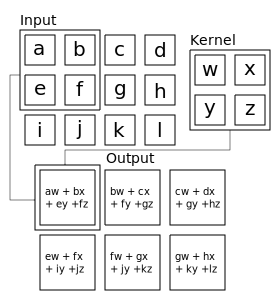
\includegraphics[scale=1]{crosscorrelation}
 \caption{2-D convolution.}
 \label{fig:crosscor}
\end{figure}

Figure ~\ref{fig:crosscor} show how a 2-D convolution takes place with no kernel-flipping. It can also be noticed that due the smaller kernel size, the convolution operation correspond to a sparse matrix. Most Neural Network models allow to easily replace a matrix multiplication with a convolution (as long as the model does not depend on specific matrix structures).
Convolution can be seen as a multiplication by a matrix, nevertheless the matrix has its entries constrained . For unidimensional convolution this is known as \textit{Toeplitz matrix}.For a 2-D convolution operation the \textit{doubly block circular matrix} is the analogue.  
Convolution can be seen as multiplication by a matrix with several constrained entries (e.g. Univariate discrete convolution is constrained to be a \textit{Toeplitz matrix}).
A convolution in two dimensions corresponds to a \textit{doubly block circular matrix}. 

Typical CNN models make use of more specialized stages in order to deal with large data inputs. These stages perform different operations and together form a \textit{Convolutional layer}. Convolutional layers are explained in the following subsection ~\ref{sub:convmod}.

\subsubsection{Variants of the Convolution function}
As explained in the past section ~\ref{subsec:convop}, the functions used in CNNs differ slightly from the convolution operation in the mathematical literature. 
First of all, there are several convolution operations which run in parallel, this is due the kernel properties. A kernel can only extract one kind of features, therefore multiple convolutions in a layer help to obtain many kind of features.
Also the inputs are generally a grid of vector-based observations rather than real values. When working with images, the inputs and outputs are represented as 3-D tensors, with one index for the different channels (i.e. red, green and blue) and the other two indices for the spatial coordinates.
In equation ~\ref{equ:varconv}, ${K_{i,j,k,l}}$ is the kernel, which gives the connection strength between a unit in channel \textit{i} of the output and a channel \textit{j} of the input, with an offset of \textit{k} rows and \textit{l} between the output and the unit. The input data is formed by the elements ${V_{i,j,k}}$, where \textit{i} indicates the channel and \textit{j} and \textit{k} indicate  rows and columns respectively. The convolution is assumed without kernel flipping. 

\begin{equation}
 {Z_{i,j,k}} = \sum_{l,m,n}{V_{l,j+m,k+n}}{K_{i,l,m,n}}
 \label{equ:varconv}
\end{equation}

In order to reduce computational costs, it is possible to skip over some positions of the kernel (the feature extraction becomes coarse). It can be seen as a downsampling in the convolution and appears in equation ~\ref{equ:downconv}. The \textit{s} is referred as the stride and allows to sample only every \textit{s} pixels in each direction of the output.

\begin{equation}
 {Z_{i,j,k}} = \sum_{l,m,n}[{V_{i,j \times s+m,k \times s+n}}{K_{i,l,m,n}}]
 \label{equ:downconv}
\end{equation}

Zero-pad is one essential feature of the convolution that should be implement at the input in order to make it wider. The width of the representation is reduced by the kernel width - 1 at each layer if zero padding is not implemented. Therefore zero padding avoids the necessity to choose between shrinking the spatial representation and using small kernels. 

In order to perform learning in a convolutional neural network, other operations are required. A Computation of gradients with respect to the kernel, given the gradients with respect to the output must be yield. 

\begin{figure}
 \centering
 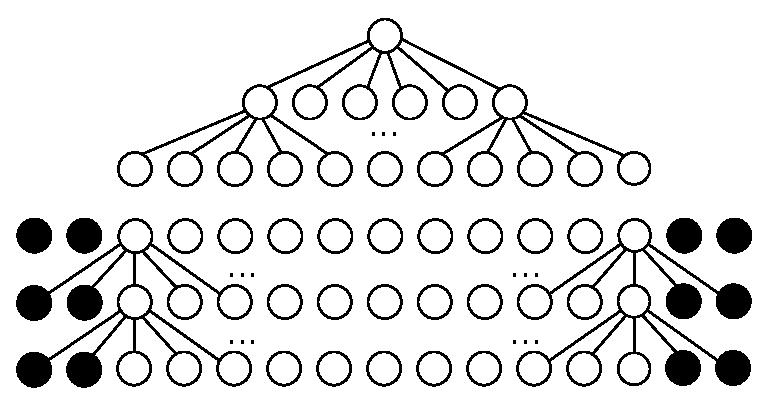
\includegraphics[scale=1]{zero-padding}
 \caption{\textit{Zero Padding effect:} \textbf{TOP:} Zero padding is not implemented,, therefore the network shrinks its size. \textbf{BOTTOM:} Zero padding prevents the network from shrinking with depth.}
 \label{fig:zp}
\end{figure}

\subsection{Convolutional Layer}
\label{sub:convmod}
CNN models are composed of several layers, where at least one of them is a \textit{convolutional layer}. Convolutional layers have these stages:
\begin{itemize}
 \item Convolution stage
 \item Detector stage
 \item Pooling stage
 \item (Local Response Normalization stage)
\end{itemize}

The norm stage appears in brackets because it is not always present in a convolution layer. However, it is present in several architectures. Figure ~\ref{fig:convlay} shows how all the stages inside a convolutional layer are interconnected. The convolution stage is already explained in ~\ref{subsec:convop} and the rest of the stages are explained below.
  
\begin{figure}
 \centering
 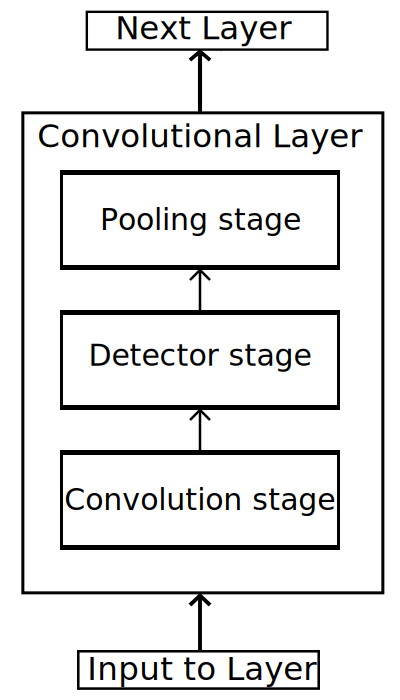
\includegraphics[scale=0.3]{convolutional_layer}
 \caption{Each convolution layer is divided into three stages.}
 \label{fig:convlay}
\end{figure}

\subsubsection{Detector stage}
\label{subsub:detector}
In the detector stage an \textit{activation function} is performed. An activation function defines an output for a given input or set of inputs. There are three main kinds of activation functions:
\begin{itemize}
 \item \textit{Hyperbolic tangent function (Tanh)}:
  \begin{equation}
   f(x) = \frac{e^{x}-e^{-x}}{e^{x}+e^{-x}}
   \label{equ:tanh}
  \end{equation}
 \item \textit{Logistic sigmoid function}:
   \begin{equation}
    f(x) = \frac{1}{ 1 + e^{-x}}
    \label{equ:sigmoid}
   \end{equation}   
 \item \textit{Rectified Linear Unit function (ReLU)}:
  \begin{equation}
   f(x) = max(0,x)
   \label{equ:relu}
  \end{equation}
 \item \textit{Parametric Rectifier Linear Unit function (PReLU)}:
  \begin{equation}
  f(x) =\begin{cases} ax & \mbox{if } x \leq 0 \\ x & \mbox{if } x > 0 \end{cases}     
  \label{equ:prelu}
  \end{equation}     
\end{itemize} 

In equations ~\ref{equ:tanh}, ~\ref{equ:sigmoid}, ~\ref{equ:relu} and ~\ref{equ:prelu}; \textit{x} represents the input and \textit{f(x)} is the respective output. The behavior of each activation function can be observed in Figure ~\ref{fig:actfct}. All of these functions are widely used for deep learning, but only the last two (ReLU and PReLU) are nowadays used for Convolutional Neural Networks. Therefore \textit{tanh} and \textit{sigmoid} functions are not covered. In order to coincide with \textcite{Bengio-et-al-2015-Book} the rectifier functions will be referred as  \textit{Detector stage}.

\begin{figure}
 \centering
 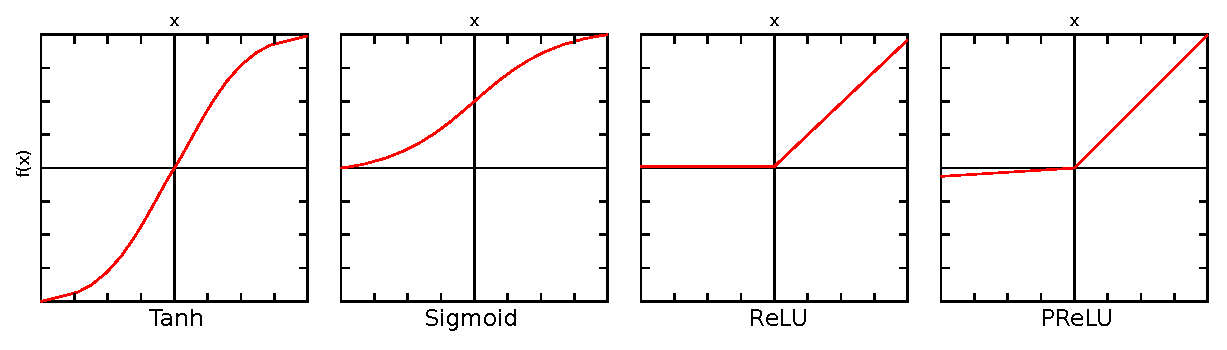
\includegraphics[scale=0.7]{activation_fct}
 \caption{The different types of activation functions used in Convnets.}
 \label{fig:actfct}
\end{figure}

% There is no clear understanding of how and why a CNN works, usually better perfomance is achieved by trial-and-error 
\textcite{zeiler2013rectified} mention and prove empirically how CNNs benefit from ReLU functions. The nature of ReLU functions allows to easily train deep networks (even from random initialization). Equation ~\ref{equ:relu} transform the system into a linear system since it only focuses on non-zero units. ReLU also yield a more regularized internal representation (zero-outputs are often produced, if there is misalignment between inputs and internal weights).   state that there are two reasons for ReLU to be beneficial for efficient learning of deep neural networks. The first reason is the system reduction to a linear convex system (it only focuses on units that are non-zero). The other reason is a more regularized internal representation. ReLU often produce zero-outputs, if the input is not aligned with the internal weights.

According to \textcite{glorot2011deep} ReLU units are suitable for CNNs due the sparsity of data, an inherent property of the convolution operation. It is worth to mention that not only vision tasks obtain a performance improvement, but also acoustic models (\textcite{maas2013rectifier}) and speech processing (\textcite{zeiler2013rectified}). It becomes obvious that Rectified Linear units are a must in order to yield state of the art results while using CNNs. 
%PReLU is trained and optimized using backpropagation (\textcite{le1990handwritten}) just as the other layers 
%\begin{equation}
% \frac{\partial \varepsilon}{\partial {a_i}} = \sum\limits_{y_i} \frac{\partial \varepsilon}%{\partial f({x_i})} \frac{\partial f({x_i})}{\partial {a_i}}
%\end{equation}

The Parametric Rectified Linear Unit (PReLU) is shown in figure ~\ref{fig:actfct} and can be seen as modified version of the ReLU function. It succesfully surpassed the performance achieved by  ReLU based CNN models (\textcite{he2015delving}). Its implementation improves model fitting with almost no extra computational effor and reducing the overfitting risk. PReLU Robustness lies in the \textit{a} parameter from equation ~\ref{equ:prelu} which is learnable. This is similar to the Leaky Rectified Linear Unit (LReLU) proposed in \textcite{maas2013}, which uses a small fixed value (\textit{a =  0.01}) to avoid zero gradients; but when comparing to ReLU only PReLU performance has a significant impact. In PReLU, only by adding few parameters with a negligible computation cost, a CNN performance is improved due the adaptative learning of activation function shapes.  
%According to \textcite{glorot2011deep}, ReLU are suitable for CNNs since they benefit from sparse data, an inherent property of the convolution operation. They proved their efficiency not only in vision tasks, but also in acoustic models (cite Maas), \textit{Restricted Bolzmann Machines (RBM)} (cite V. Nair) and also speech processing (cite Zeiler). Therefore this detector stage becomes essential for state of the art neural networks. 
%Neural Networks are special case of program paradigms. Their singularity lies inside the learning capability from observed data. Despite being invented several years ago, it was recently when they started to achieve a better perfomance than some other traditional approaches. These new techniques are the now so called deep neural networks.

%Deep Learning and Deep Neural Networks are nowadays in development and still reaching outstanding performance on many problems (i.e. Computer Vision, Speech Recognition, et cetera.)

%Convolutional Neural Networks (CNNs) process data with a grid-like topology. The name implies that a mathematical operation called "convolution" is yield. CNNs use convolution instead of general matrix multiplication. (Cite Bengio)

%For CNNS, the first argument in a convolution is called input and the second argument is referred as kernel. The output is known as Feature Map.

%Inputs are usually multidimensional arrays of data and Kernels are mutlidimensional array of parameters that can be learned.

%CNNS have sparse interactions "sparse connectivity/weights" due a kernel smaller than the input. This allows to save fewer parameters, reduces memory requirements and improves statistical efficiency 

%insert ReLU eps and tanh, sigmoid function plots

\subsubsection{Pooling stage}
\label{subsub:pool}
As shown in figure ~\ref{fig:convlay}, the convolution layer is formed of convolution, detector and pooling stage. The pooling stage modifies the output of the layer further. It replaces the output in a certain location with a statistical summary of the nearby outputs. 
The Pooling stage comes after the Detector stage. It replaces the output in a certain location with a statisctial summary of the nearby outputs. Its purpose is to reduce the invariance caused by small translations inside the inputs. The most common pooling functions are:

\begin{itemize}
 \item \textit{Max function}: Maximum output within a rectangular neighborhood.
 \item \textit{L2 norm function}: Squared root of the absolute values squared.
 \item \textit{Average function}: Average output of a rectangular neighborhood.
 \item \textit{Weighted average function}: Output based on the distance from the central pixel.
\end{itemize}

Invariance to local translation has been proved to be an important property if the vision task focuses more on the presence of a feature rather than in its location. However depending on the task to preserve the location of a feature is desired.
Pooling summarizes over an output neighborhood allow to use fewer pooling stages than detector stages . Figure ~\ref{fig:maxpool} shows how this summarization generates an increased computer efficiency and reduced memory requirements because the next layer will have fewer parameters to process. The figure depicts a max-pooling operation with a pool width of three and a stride between pools of two. 

Convolution and Pooling can cause underfitting, therefore state of the art models (e.g \textcite{Krizhevsky_imagenetclassification} and \textcite{szegedy2014going}) are designed to use pooling on some channels. This yields highly invariant features and features which are non prone to underfitting

\begin{figure}
 \centering
 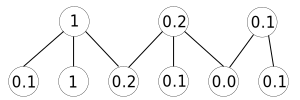
\includegraphics[scale=1]{maxpooling}
 \caption{Pooling with downsampling}
 \label{fig:maxpool}
\end{figure}

\subsubsection{Local Response Normalization (LRN)}
\label{subsub:LRN}
Response normalization is implemented as a form of lateral inhibition, and is inspired on the real neurons. \textcite{hinton2012improving} introduced this type of layer in order to encourage competition for large activations amongst neuron outputs which are computed using different kernels. In order to yield a better generalization, the local normalization is performed as in equation ~\ref{equ:LRN}.$b^i_{x,y}$ represents the  response-normalized activity, $a^i_{x,y}$ denotes the activity of a computed neuron, where $i$ is the kernel and $(x,y)$ the position coordinates. The sum runs over $n$ kernel maps at the same spatial position and $N$ stands for the number of kernels in the layer.  

\begin{equation}
 b^i_{x,y} =  a^i_{x,y}/ \bigg( k+\alpha\sum\limits_{j=max(0,i-n/2)}^{min(N-1,i+n/2)}(a^j_{x,y})^2 \bigg) ^\beta
 \label{equ:LRN}
\end{equation}

The constanst $k$,$n$,$\alpha$ and $\beta$ are hyperparameters which are calculated using a validation set. A LRN layer follows a ReLU layer, though ReLU units do not require input normalization, but as \textcite{Krizhevsky_imagenetclassification} implemented it prevents saturating inputs.
  
\subsection{Deconvolutional Layer}
\textcite{zeiler2011adaptive} proposes this novel architecture which uses the same components of a convolutional layer (See section ~\ref{sub:convmod}) but in reverse. Originally used to perform unsupervised learning, the deconvolutional layers are later used as a visualization technique in CNNs. This approach appears in \textcite{zeiler2014visualizing}. It allows to to find the performance contribution of a layer, and have also been used in image segmentation tasks (e.g. \textcite{long2014fully}, \textcite{noh2015learning}) 

Equation ~\ref{equ:deconv} shows how the reconstruction $\hat{y_1}^c$, where $c$ represents the color channels, is performed by the sum of  convolution operations of the feature maps $z_{k,1}$ with filters $f^c_{k,1}$. 
\begin{equation}
 \hat{y_1}^c = \sum\limits_{k=1}^{K_1}z_{k,1}\ast f^c_{k,1}
 \label{equ:deconv}
\end{equation}

The deconvolution tries to minimize the reconstruction error under a sparsity constraint and a set of feature maps. This is explained in equation ~\ref{equ:deconvcost}. $C_l(y)$ stands for the cost function and comprises two terms weighted by $\lambda_l$ a likelihood which keeps the $\hat{y}_t$ reconstruction close to $y$ input, and a regularization term of the feature maps $z_{k,l}$. 
 
\begin{equation}
 C_l(y) = \frac{\lambda_l}{2} ||\hat{y}_l-y||^2_2+\sum\limits_{k=1}^{K_t}|z_{ĸ,l}|_1
 \label{equ:deconvcost}
\end{equation}

Figure ~\ref{fig:deconv} explains how a deconvolutional layer works. The activities performed in a convolutional layer are mapped back to the pixel space. The stages are performed successively in this order: unpooling, rectifying and filter.

\begin{figure}
 \centering
 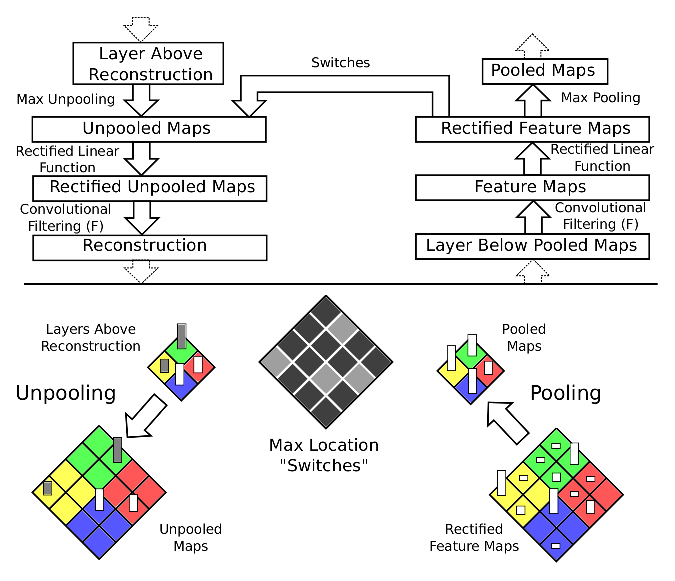
\includegraphics[scale=1]{deconvolution}
 \caption{\textbf{LEFT}: deconvolutional layer. \textbf{RIGHT}: convolutional layer. The deconvolution layer yields an approximate reconstruction of the layer beneath convolution layer.
 \textbf{BOTTOM}: This diagram depicts the unpooling operation in the deconvolutional layer. The black/gray squares are negative/positive activations in the feature map (\textcite{zeiler2014visualizing}).}
 \label{fig:deconv}
\end{figure}

\section{Convolution parameters}
\subsubsection{Dropout}
Another addition to the convolutional neural networks is the so called \textit{dropout layer}. Deep neural nets are characterized for having a large number of parameters, therefore the nets are prone to overfitting. In order to address the overfitting problem, there are several techniques that can be implemented (e.g. soft weight sharing, penalties like L1 and L2 regularization, stop the training if the performance in the validation data is reduced).

It is possible to "regularize" a model by averaging the predictions of all possible setting of the parameters. This works well for small models, however the use of this technique on a several number of learned models that share parameters (i.e. Model combination) is computationally expensive.
 
\textcite{srivastava2014dropout} proposed the \textit{Dropout} technique in order to address the two cited problems (i.e. overfitting and high computational effort). It also allows to combine many different neural networks architectures in an efficient way. Figure ~\ref{fig:dropout} depicts the dropout technique, which can be define as the drop out  of units in a neural network.  Normally each unit is retained with a fixed probability \textit{p} (usually set at 0.5) in order to be optimal for many kinds of networks and tasks. A Neural Network trained with the dropout technique can be seen as a collection of $2^n$ thinned networks, each of which shares its weights. 

\begin{figure}
 \centering
 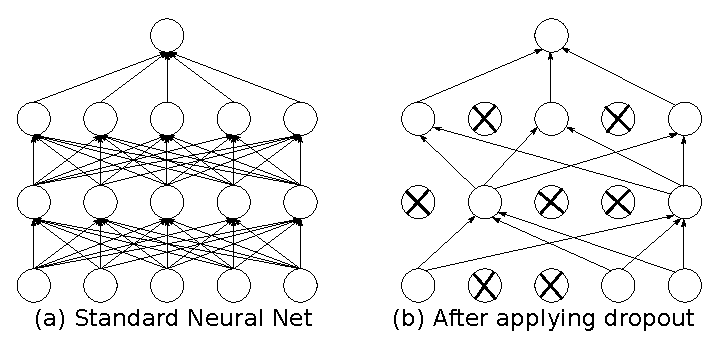
\includegraphics[scale=1]{dropout}
 \caption{\textbf{Left}: A standard neural net with 2 hidden layers. \textbf{Right}: An example of a thinned net, producht of the dropout technique.}
 \label{fig:dropout}
\end{figure}

A model where dropout is performed can be described as follows: Given \textit{L} hidden layers, let $l\in\{1,...,L\}$ index the hidden layers. $z^l$ and $y^l$ are vectors of inputs into layer $l$ and outputs from layer $l$ respectively. $w^l$ and $b^l$ represent the weights and biases at layer $l$. Feed forward operation of a standard neural network is then described in equations ~\ref{equ:do1} and ~\ref{equ:do2}.
  
\begin{equation}
 {z_i}^{(l+1)} = {w_i}^{(l+1)}y^l+{b_i}^{(l+i)}
 \label{equ:do1}
\end{equation}

\begin{equation}
 {y_i}^{(l+1)} = f({z_i}^{(l+1)})
 \label{equ:do2}
\end{equation}

where $f$ is an activation function, like the ones seen in the detector section ~\ref{subsub:detector}. The feed-forward operation in a network where dropout looks like this:  

\begin{equation}
 {r^l_j} \sim Bernoulli(p)
 \label{equ:do3}
\end{equation}

\begin{equation}
 \tilde{y}^l = r^l \ast y^l
 \label{equ:do4}
\end{equation}

\begin{equation}
 {z_i}^{(l+1)} = {w_i}^{(l+1)}\tilde{y}^l+{b_i}^{(l+1)}
 \label{equ:do5}
\end{equation}

\begin{equation}
 {y_i}^{(l+1)} = f({z_i}^{(l+1)})
 \label{equ:do6}
\end{equation}

Equation ~\ref{equ:do3} shows a $r^l$, which is a vector of random variables that have a probability $p$ of being 1. In equation ~\ref{equ:do4}, $\ast$ denotes an element-wise product. The vector $r^l$ is sampled and multiplied with the outputs $y^l$ of that layer, to create a thinned output $\tilde{y}^l$. This process is applied at each layer and the outputs are used as inputs for the next layer.

The training of the dropout units is similar to the Stochastic Gradient Descent method used in standard neural networks. Forward and backpropagation are done on the thinned networks, while the gradients for each parameter are averaged over the training cases. Momentum, annealing learning rates and L2 weight decay are also useful to omprove the stochastic gradient descent. The noise generated by the dropout allows the optimization to be most robust by exploring different regions of the weight space. 

It must be noticed that dropout introduces noise in the gradients if compared to the standard stochastic gradient descent (i.e. some grandients cancel each other). In order to overcome this issue, the learning rate should be increased 10-100 times and a high momentum must be chosen. This increase the speed of the learning process.

Nevertheless, the dropout technique in neural network has its drawbacks. The training process is 2-3 longer due a very noisy parameter update. Each training case focuses on a specific random architecture, therefore the calculated gradients are not the same gradients used in the final architecture. There is a trade-off between training time and overfitting that should be analyzed depending the characteristics of a given neural network (i.e. dataset, architecture).    

\subsection{Learning}
The forward pass and backward propagation are the main operations being yield in a neural network.

The forward pass computes the output given the input for inference.
\begin{equation}
 fw(x) = h(g(x))
 \label{equ:FWD}
\end{equation}

The backward pass \textit{(back-propagation)} computes the gradients given the loss for learning

\begin{equation}
 \frac{\partial{fw}}{\partial{h}} \frac{\partial{fw}}{\partial{W_{ip}}} \frac{\partial{fw}}{\partial{g}}
\end{equation}

\begin{figure}
 \centering
 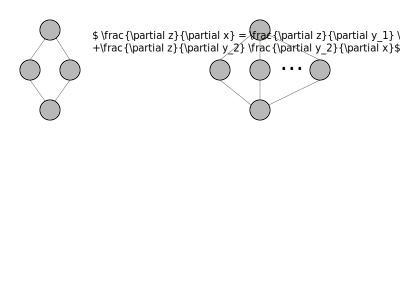
\includegraphics[scale=1]{backprop}
 \caption{backpropagation}
\end{figure}
\subsubsection{Loss functions}
\label{sec:loss}
A loss function evaluates the quality of the learning by mapping parameter settings to a scalar value, to test the \textit{accuracy} of the learned parameters. The goal of the learning process is to find a set of parameters which minimizes the loss function.

When Neural Network models started to become popular, the most used loss function was the Least Squared Error (LSE) $L(f_w(x),y) = ||f_w(x)-y||^2$. Nevertheless this is not effective if the values of $y$ are discrete (i.e. classification tasks), and therefore other loss functions should be employed.

\subsubsection{Softmax}
\label{sec:softmax}
\begin{equation}
 p = softmax(a) \Longleftrightarrow p_i = \frac{e^{a_i}}{\sum_j e^{a_j}}
 \label{equ:softmax}
\end{equation}

Equation ~\ref{equ:softmax} is the \textit{softmax} (\textcite{bridle1990probabilistic}) and its purpose is to specify multiple Bernoulli (\textit{multinoulli}) distributions. Where $a$ is a set of activations 

The softmax loss layer is conceptually identical to the softmax layer applied before a multinomial logistic layer. It is the loss function used in Caffe



\subsection{Optimization}
The backward pass defines how to compute the gradient of the loss with respect to the model parameters. However, in order to update the weights of a Neural Network, gradient-based learning algorithms need to be implemented. 
Though several learning algorithms for deep neural networks exist, this thesis only covers some of them due their popularity and therefore further implementation in Caffe
\subsubsection{Stochastic Gradient Descent (SGD)}
\label{subsub:SGD}
Stochastic Gradient Descent is a widely used optimization algorithm for machine learning. It uses a stochastic estimator of the gradient in order to perform an update.  

\textit{empirical risk} $E_n(f)$ measures the training set performance, while the \textit{expected risk} $E(f)$ calculates the expected performance on future examples. Both appear in equation ~\ref{equ:risk}
\begin{equation}
 E(f)= \int l(f(x),y)dP(z) \hspace{2cm} E_n(f) = \frac{1}{n}\sum\limits_{i=1}^nl(f(x_i),y_i)
 \label{equ:risk}
\end{equation}
Gradient Descent (GD) minimizes the empirical risk $E_n(f_w)$. In each iteration the weights $w$ on $E_n(f_w)$ are updated as in equation ~\ref{equ:1GD}:
\begin{equation}
 w_{t+1} = w_t-\gamma\frac{1}{n}\sum\limits_{i=1}^n\nabla_wQ(z_i,w_t),
 \label{equ:1GD}
\end{equation}
$\gamma$ represents the learning rate, which achieves \textit{linear convergence} in case of being sufficiently small and in conjunction with a $w_o$ close to the optimum.
If the scalar learning rate $\gamma$ is replaced by a positive matrix $\Gamma_t$ a better optimization can be designed. Equation ~\ref{equ:2GD} shows a \textit{second order gradient descent}. 
\begin{equation}
 w_{t+1}= w_t-\Gamma_t\frac{1}{n}\sum\limits_{i=1}^{n}\nabla_wQ(z_i,w_t).
 \label{equ:2GD}
\end{equation}

Stochastic Gradient Descent is a widely used optimization algorithm for machine learning. It uses a stochastic estimator of the gradient in order to perform an update. It is also known as \textit{online gradient descent} . It is a drastic simplification since each iterations estimates the gradient based on single random $z_t$:
\begin{equation}
 w_{t+1} = w_t - \gamma_t \nabla_w Q(z_i,w_t)
 \label{equ:SGD}
\end{equation}
The SGD optimizes the expected risk, due the fact that the examples are randomly drawn from a ground truth distribution. The randomly drawn examples introduces noise, therefore the SGD gradient does not become 0 even when a minimum is reached.

The learning rate $\gamma_t$ is a crucial hyperparameter, which sometimes must be allowed to decrease its size in order to converge to a minimum. 

Since the data sizes grow faster than the processing speed, Stochastic Gradient Descent have become popular. This is due its performance, which is good enough if the training time is the bottleneck.

\begin{equation}
 w_{t+1}=w_t-\gamma_t\Gamma_t\nabla_wQ(z_t, w_t)
 \label{equ:2SGD}
\end{equation} 

\begin{center}
\begin{tabular}{| l |}
\hline
 \textbf{Stochastic Gradient Descent (SGD)}\\
\hline
 \textbf{Require:} Learning rate $\gamma_t$\\
 \textbf{Require:} Initial parameter $w_t$\\
 \hspace{1cm}\textbf{while} Stopping criterion not met \textbf{do}\\
 \hspace{2cm}Sample a minibatch of $t$ examples from the training set $\textbf{z}_{(1)} ,...,        \textbf{z}_{(t)}$ \\
 \hspace{2cm}Set \textbf{$f(t) = 0$}\\
 \hspace{2cm}\textbf{for} i = 1 to $t$ do\\
 \hspace{3cm}Compute gradient estimate: $f(t+1) = f(t) + \nabla_w Q(z_i,w_t)$\\
 \hspace{2cm}\textbf{end for}\\
 \hspace{2cm}Apply update: \textbf{$w_{t+1} = w_t - \gamma_t f(t+1)$}\\
 \hspace{1cm}\textbf{end while}\\
\hline
\end{tabular}
\end{center} 

\textbf{Table with SGD Algorithm}
\textcite{bottou2012stochastic} \textcite{Bengio-et-al-2015-Book} \textcite{Krizhevsky_imagenetclassification} 

\subsubsection{Momentum}
\label{subsub:moment}
Momentum helps to overcome inherent weaknesses of the stochastic gradient descent strategy. One of the main drawbacks of SGD is the slow training time, which is particularly slow when the gradient is small. 

Momentum function is to speed up the learning process 

\begin{center}
\begin{tabular}{| l |}
\hline
 \textbf{Stochastic Gradient Descent (SGD) with momentum}\\ 
\hline
 \textbf{Require:} Learning rate $\gamma_t$, momentum parameter $\alpha$\\
 \textbf{Require:} Initial parameter $w$, inivital velocity $v$\\
 \hspace{1cm} \textbf{while} Stopping criterion not met \textbf{do}\\
 \hspace{2cm} Sample a minibatch of $t$ examples from the training set  $\textbf{z}_{(1)} ,...,        \textbf{z}_{(t)}$ \\
 \hspace{2cm} Set $\textbf{f(t) = 0}$\\
 \hspace{2cm} \textbf{for} $i=1$ to $t$ \textbf{do}\\
 \hspace{3cm} Compute gradient estimate: $f(t+1) = f(t) + \nabla_w Q(z_i,w_t) $\\
 \hspace{2cm} \textbf{end for}\\ 
 \hspace{2cm} Compute velocity update: \textbf{$v = \alpha v-\gamma_t f(t+1)$}\\
 \hspace{2cm} Apply update: \textbf{$w_{t+1} = w_t + v$}\\
 \hspace{1cm} \textbf{end while}\\
\hline
\end{tabular}
\end{center}



\subsubsection{Adaptative Gradient (AdaGrad)}
\label{subsub:AdaGrad}

The AdaGrad algorithm scales the learning rates of all parameters inversely proportional to a sum of squared partial derivates over the iterations in order to adapt them individually.  A rapid decrease in the learning rate corresponds to the parameters with large partial derivative of the loss. This yields a greater advance in the more sloped directions of parameter space.

The use of AdaGrad has a drawback if it is applied to deep neural networks. Due  an accumulation of squared gradients,  results in a premature and excessive decrease in the learning rate. The AdaGrad algorithm is explained in  ~\ref{tab:AdaGrad}.

\begin{center}
\begin{tabular}{| l |}
\hline
\textbf{AdaGrad algorithm}\\
\hline
\textbf{Require:} Global learning rate $\gamma$,\\
\textbf{Require:} Initial parameter $w_t$\\
 \hspace{1cm} Initialize gradient accumulation variable \textbf{$r=0$}\\
 \hspace{1cm} \textbf{while} Stopping criterion not met \textbf{do}\\
 \hspace{2cm} Sample a minibatch of $t$ examples from the training set $\textbf{z}_{(1)} ,...,        \textbf{z}_{(t)}$ \\
 \hspace{2cm} Set \textbf{$f(t) = 0$}\\
 \hspace{2cm} \textbf{for} $i=1$ to $t$ \textbf{do}\\
 \hspace{3cm} Compute gradient: \textbf{$f(t+1) = f(t) + \nabla_w Q(z_i,w_t)$}\\
 \hspace{2cm} \textbf{end for}
 \hspace{2cm} Accumulate gradient: \textbf{$r = r^2+f^2(t+1)$} \\
 \hspace{2cm} Compute update: \textbf{$\Delta w_t = \frac{\gamma_t}{\sqrt{r}} f(t)$}\\
 \hspace{2cm} Apply update: \textbf{$w_{t+1} = w_t + \Delta w_t$}\\
 \hspace{1cm} \textbf{end while}\\
\hline
\end{tabular}
\label{tab:AdaGrad}
\end{center}
\textcite{Bengio-et-al-2015-Book} \textcite{duchi2011adaptive}
\subsubsection{Nesterov's Accelerated Gradient (NAG)}
\label{subsub:NAG}
\begin{center}
\begin{tabular}{| l |}
\hline
\textbf{Stochastic Gradient Descent (SGD) with Nesterov Momentum}\\
\hline
\textbf{Require:} Learning rate $\gamma$, momentum parameter $\alpha$.\\
\textbf{Require:} Initial parameter $w_t$, initial velocity $v$.\\
\hspace{1cm} \textbf{while} Stopping criterion not met \textbf{do}\\
\hspace{2cm} Sample a minibatch of $t$ examples from the training set $\textbf{z}_{(1)} ,...,        \textbf{z}_{(t)}$ \\
\hspace{2cm} Apply interim update: \textbf{$w_{t+1} = w_t + \alpha v$}\\
\hspace{2cm} Set \textbf{$f(t) = 0$}\\
\hspace{2cm} \textbf{for} $i = 1$ to $t$ \textbf{do}\\
\hspace{3cm} Compute gradient (at interim point): \textbf{$f(t+1) = f(t) + \nabla_w Q(z_i,w_t)$}\\
\hspace{2cm} \textbf{end for}\\
\hspace{2cm} Compute velocity update: \textbf{$v = \alpha v - \gamma_t f(t+1)$}\\
\hspace{2cm} Apply update: \textbf{$w_{t+1} = w_t + v$}\\
\hspace{1cm} \textbf{end while}\\
\hline
\end{tabular}
\end{center}

\textcite{nesterov1983method} \textcite{sutskever2013importance}

%Color image data: One channel per color (RGB) while the kernel moves over horizontal an vertical axes.

\section{CNN outputs}
CNN models have structured outputs.
To achieve classification on a pixel level, in order to perform an image segmentation like in \textcite{farabet2013pami}. There is a trade-off due the pooling layers, since they subsample the feature maps and therefore they are skipped in some levels.
\section{Classifiers}

\subsection{AlexNet}
AlexNet is a classifier that won ImageNet Large-Scale Visual Recognition Challenge 2012 (ILSVRC12). (Cite ImageNet paper) 
The AlexNet architecture is shown in Figure . It has five Convolution Layers and three Fully Connected Layers. In order to train the AlexNet architecture, a dataset consisting in 1.2 million images representing 1000 categories is used.
The output of its neurons is modelled by  Rectified Linear Units (ReLU), which satisfy the non-saturating nonlinearity function \(f(x) = max(0,x)\).

CNNs that use ReLU instead of other equivalents (e.g. tanh and sigmoid functions) train several times faster. It would not be possible to train large networks with the traditional saturation models such as the previously mentioned functions. 
Local Response Normalization (LRN) is present, because it aids generalization. Nevertheless ReLU prevent saturation for themselves.
Pooling layers are contained to summarize the output of neighboring neurons in a statistical representation. In order to have an overlapping pooling, Stride value is set to two. This have shown to avoid overfitting during training.
This network has 1000 non-spatial class labels. The output of the last fully connected layer is fed to a softmax layer which produce a distribution over the class labels.

The AlexNet includes the Dropout techinque (cite dropout paper), in which the output of each hidden neuron is given the value zero with a probability of 0.5. These neurons are "dropped out" and therefore do not take part in backpropagation and do not participate in the forward pass. This technique makes neurons unable to rely on the presence of  particular neurons. Dropout encourages learning of robust features whoch are useful with different subsets of neurons in conjunction. There is a tradeoff within the Dropout technique: By decreasing the overfitting, the number of iterations needed to converge is doubled.

The Details of learning.
This model is produced using Stochastic Gradient Descent (SGD) algorithm with a batch size of 128 images, the momentum of 0.9 and the weight decay of 0.0005. The weight decay is important for the network architecture to learn, since it reduces the network's training error.
Zero-mean Gaussian distributions with a standard deviation of 0.01 are used to initialize the weights. The biases for the hidden layers are initialized with the constant 1 in the second, fourth and fifth Convolutional Layers, and in all fully connected layers; the remaining layers are initialized with a bias equal to the constant 0. The initial learnng rate is 0.01 and it gets divided by 10 when the validation error stops improving. 
%insert Alexnet eps image 
\subsection{GoogLeNet}
GoogLeNet participated and performed well in the ILSVRC14. Its results for classification and detection are the state of the art.It consist of 22 layers.
Remarkable is that this network uses several times fewer parameters in comparison with other CNNs. In order to accomplish this a 22 layers architecture was designed with an intention to increase the network depth. This new concept is denominated "Inception". The main idea of the Inception architecture is to find an optimal local sparse structure using readily available components.

Traditional methods tend to increase the size of deep neural networks to improve their performance. However such an increase in size also has its drawbacks: The network has more parameters which makes it more prone to overfitting if the training data is not sufficient; the increase in size implies an increased use of computation resources. The GoogLeNet overcomes this problem in a more efficient way with its "Inception" technique which avoids the inherent problems in size increase.
The network is divided into "Inception Modules" which are stacked in top of each other. They are shown in Figure.

This Inception approach was first proposed by (cite Lin et al). It basically adds 1x1 convolutional layers. 1x1 convolutional layers help to remove computational bottlenecks  by dimension reduction. Figure b  shows how this dimension reduction allows to deal with the prohibitively expensive 5x5 convolutions inside the "Inception Modules" while keeping the computational requirements expensive.
In ordert to save computational budget and to increase the quality of the results, the GoogLeNet architecture is sparsely connected.

The GoogLeNet consists if these "Inception Modules" stacked upon each other. Max-pooling layers appear occasionally to halve the grid resolution.  It must be noticed that the "inception modules" only appear in the higher layers, while the lower layers present a traditional convolutional approach. ReLU is the activation function for all the convolutions. In order to enable fine-tuning and adaptation of this network an extra linear layer was added. Dropout for GoogLeNet has a 70 percent ratio. The training method relies on Stochastic Gradient Descent (SGD), a 0.9 momentum  and a fixed learning rate (it decreases 4\% every 8 epochs). 
% include inception module eps image

\section{Semantic Segmentation}
\label{sec:secseg}

The invariance to local translation is important for vision tasks where the presence of a feature  rather than exact location is required.

Classifiers

Y. Lecunn (cite) created the modern CNNs in 1989

\section{Efficient based graph segmentation}
\label{sec:effi}
This algorithm yields a segmentation based on a graph-based approach and is contained in \textcite{felzenszwalb2004efficient}. The \textit{Efficient based graph segmentation} algorithm considers pixels as vertices (\textit{v}) and the dissimilarity between two  neighboring pixels (\(v_{i} , v_{j}\)) as edges. The image is considered as an undirected graph \(G = (V,E)\) where \(V\) is the set of vertices (\(v \in V\) and \(E\) is the set of edges (\(v_{i} , v_{j}\in E\)). Each edge (\(v_{i} , v_{j}\)) has a corresponding weight (\(w(v_{i} , v_{j})\) which measures the dissimilarity (e.g color, intensity, motion, etc.).

A segmentations is induced by a subset of edges. This means that a segmentation \textit{S} partitions the set \textit{V} into components which correspond to \(G'=(V,E')\) such that \(C \in S\) and \(E' \subseteq E\). The main criterion to define a segmentation is to have similar elements in a component \textit{C}. According to this criterion, edges between two elements in a component have low weights, while two edges between elements in different components must have higher weights.

A predicate \textit{D} should be defined to evaluate if a boundary between two components is present (two regions in an image). The resulting predicate makes a comparison between the inter-component difference and the internal difference within the components. The predicate is therefore adaptive with respect to the local characteristics of data.

The \textit{Internal difference} of a component \(C \subseteq V\) is defined as the largest weight in the minimum spanning tree of the component itself (\(MST(C,E)\)). It is defined in the equation ~\ref{equ:mst} :

\begin{equation}
 Int(C) = \max_{e \in MST(C,E)} w(e)
 \label{equ:mst}
\end{equation}

The \textit{difference between two components} is the minimum weight edge connecting these components. It is defined as follows: 

\begin{equation}
 Dif(C_{1},C_{2}) = \min_{v_{i} \in C_{1} , v_{j} \in C_{2} , (v_{i},v_{j}) \in E} w(v_{i},v_{j})
\end{equation}

In case that no edge is connecting \(C_{1}\) and \(C_{2}\), the difference is considered to be infinite (\(Dif(C_{1},C_{2}) = \infty\)). This criterion could be changed but it would modify the difficulty of the problem.
In order for the region comparison to work, a threshold function must be used to check if evidence of a boundary between a pair of components exists. The pairwise comparison is shown in ~\ref{equ:comp}

\begin{equation}
 D(C_{1},C_{2}) = \begin{cases} \mbox{true} & \mbox{if } Dif(C_{1},C_{2}) > MInt(C_{1},C_{2})\\ \mbox{false} & \mbox{otherwise} \end{cases}
 \label{equ:comp}
\end{equation}

However the size of a component is irrelevant to this definition. A threshold function \(\tau\) must be defined to control the internal difference taking into account the component size.
By adding this threshold to ~\ref{equ:comparison}, the next equation is obtained:

\begin{equation}
 MInt(C_{1},C_{2}) = \min (Int(C_{1})+\tau(C_{1}),Int(C_{2})+\tau(C_{2}))
\end{equation}

where:

\begin{equation}
 \tau(C) = k/|C|
 \label{equ:tap}
\end{equation}

In equation ~\ref{equ:tap}, \(|C|\) is the size of \(C\) and \(k\) is a constant parameter.
A larger \(k\) value causes a preference for larger components. 

A Gaussian filter is used to remove small artefacts product of the digitization. The Gaussian filter is set with a \(\sigma = 0.8\), it smooths the image before computing the edge weights.

An extra parameter \(t\) can be set, in order to remove small and undesired components. It defines a minimum size of the components and enforces those components which are too small to be joined with their nearest neighbor.

This algorithm can yield a segmentation that is neither too coarse nor too fine. This is done by changing the \(k\), \(\sigma\) and \(t\) parameters. 

The 	\textit{Efficient graph-based segmentation} is a fundamental part of the Causal Segmentation algorithm found in \textcite{couprie2013causal} which is going to be described later in this chapter.
\subsection{Watershed cuts}
\label{subsec:watershed}
The idea of watershed comes from topography: a drop of water which falls on a surface reaches the minimum by following a descending path. It can be definded as separating lines of the domain of attraction of drops of water. This notion is applied in an edge weighted-grap.

The regions of a watershed (\textit{Catchment basins}) are the regional minima of the map. Each catchment basin contains a unique regional minimum and each regional minimum is included in a unique catchment basin.
Edge-weighted graphs
The concept of edge-weighted graphs is explained in ~\ref{sec:effi}
\(F\) is a set of all maps from \(E\) to \(Z\) and  
Watershed-cuts by the drop of a water principle:
%\(\pi = (x_{0},..,x_{l})\) be a üath in \(G\). The path \pi descends \(for F\) if, for any \(i\) \in [1,l-1], F({x_{i-1},x_{i}})\geq F(({x_{i},x_{i+1}). 
The \textit{Minimum Spanning Forest} algorithm is explain in Table ~\ref{tab:msf}
\begin{center}
 \begin{tabular}{| c |}
 \hline
 Minimum Spanning Forest algorithm \\
 \hline
 \textbf{Data:} A weighted graph \(G(V,E)\) and a set of labeled \\
  nodes markers \(L\). Nodes of \(V \textbackslash L \) have unknown \\
  labels initially.\\
 \textbf{Result:} A labeling \(x\) associating a label to each vertex. \\
Sort the edges of \(E\) by increasing order of weight.\\
 \textbf{while} \textit{any node has an unknown label} \textbf{do} \\
 Find the edge \(e_{ij}\) in \(E\)of minimal weight; \\
 \textbf{if} \(v_{i} or v_{j} have unknown label values\) \textbf{then} \\
  Merge \(v_{i}\) or \(v_{j}\) into a single node, such that\\
  when the value for this merged node becomes\\
  known, all merged nodes are assigned the\\
  same value of \(x\) and considered known.\\ 
 \hline
 \end{tabular}
% \caption{Table xx: The pseudo code for the minimum spanning forest algorithm}
 \label{tab:msf}
\end{center}


\subsection{Optical Flow}
Optical Flow infers information about motion within a scene over time. \textcite{horn1981determining} defines the Optical Flow as the distribution of apparent velocities of movement of brightness patterns in an image. The discontinuities in the optical flow are useful to segment images into regions that correspond to different objects. 

Motion is perceived when a changing picture is projected onto a stationary screen
\begin{equation}
 \frac{dE}{dt} = 0
\end{equation}
\begin{equation}
 \frac{\partial E}{\partial x}\frac{dx}{dt} + \frac{\partial E}{\partial y} \frac{dy}{dt}+\frac{\partial E}{\partial t} = 0
\end{equation}

\[u= \frac{dx}{dt}\mbox{ and } v= \frac{dy}{dt},\]

\begin{equation}
 E_{x}u+E_{y}v+E_{t} = 0,
\end{equation}
\[E_{x},E_{y}\cdot (u,v)=-E_{t}.\]
A smoothness constraint is added since opaque objects of finite size are observed while they are subject of rigid motion or deformation.
This constraint implies that neighboring points on the objects have similar velocities and the changes in the velocity field are smooth. However when an objects occludes another a discontinuity in flow occurs.
The smoothness constraint can be expressed limiting the difference between the flow velocity at a point and the average volocity over a small neighborhood containing the point. The Laplacians of \(u\) and \(v\) are defined in equation ~\ref{equ:lapla} 
\begin{equation}
 \bigtriangledown^2u=\frac{\partial^2 u}{\partial x^2}+\frac{\partial^2 v}{\partial y^2} \mbox{ and } \bigtriangledown^2v=\frac{\partial^2 v}{\partial x^2}+\frac{\partial^2 u}{\partial y^2}
 \label{equ:lapla}
\end{equation}

\section{Causal graph-based segmentation} % Temporary consistent segmentation
\label{sec:tempconsseg}

Causal segmentation for this thesis purposes is based on \textcite{couprie2013causal}. 
In order to define markers, independent segmentations are perfomed and the produced super-pixels are matched. A final segmentation is produced using the obtained markers by minimizing a global criterion defined on the image.

A segmentation \(S_{t+1}\) at a time \(t+1\) which is consistent with a given segmentation \(S_{t}\) of an image at time \(t\).

In order to produce super-pixels, independent segmentations are done using the \textit{efficient graph-based method} explained in ~\ref{sec:effi}. These independent segmentations  will be referred as \(S'_{1}...,S'_{t}\).

After an independent segmentation \(S'_{t+1}\)  is produced , the propagation of the temporal consistency between the non overlapping contours of \(S'_{t}\) and \(S'_{t+1}\) is required. This will be addressed as \textit{Graph matching} procedure.
\begin{equation}
 w_{ij}=\frac{(|r_{i}|+|r_{j}|d(c_{i},c_{j})}{|r_{i} \cap r_{i}|} + a_{ij},
 \label{equ:graphmatch}
\end{equation}

%In equation ~\ref{equ:graphmatch} \(|r_{i}|\) denotes the number of pixels in region \(r_{i}\), \(|r_{i} \cap r_{i}|\) the  number of pixels present in \(r_{i}\) and \(r_{j}\) with aligned centroids, and \(a_{ij} the appearance difference of regions \(r_{i}\) and \(r_{j}\)(e.g. difference between mean color intensities).

%For each region of \(S'_{t+1}\) its best corresponding region in image \(S'_{t+1})\ .% In order to minimize the weight \(w_{ij}\) Every node \(i\) of \(V_{t}\) is associated with a node j of \(V’_{t+1}\)
%In order to compute the final segmentation \(S_{t+1}\) , a minimum spanning forest procedure is used. 
This causal segmentation algorithm makes use of watershed cuts found in \textcite{cousty2009watershed}. The watershed algorithm allows to reuse the sorting of edges done in  ~\ref{sec:effi} and represents the main computational effort. A detailed explanation of watershed cut algorithm is present in ~\ref{sec:watershed}

\begin{equation}
 E(x)=\sum_{e_{ij} \in E} w^p_{ij}|x_{j}-x_{i}|^q + \sum_{v_{i} \in V} w^p_{i}|l_{i}-x_{i}|^q,
 \label{equ:globopt}
\end{equation} 

\(l\) represents a given configuration and \(x\) represents a target configuration

%Once \(S_{t}\) and \(S_{t+1}\) are obtained, an optical flow map can be easily computed from both segmentations. for each label \(r\) present in region \(r\) from \(S_{t+1}\) and coming from region \(s\) in \(S_{t}\) respectively, the optical flow in \(r\] can be calculated as the distance bewteen the centroid of \(r\) and the centroid of \(s\). 
 
%Intermediate-level vision problems (e.g. motion estimation require an appropriate region of support) There is a need of non-uniform region identification and segmentation techniques yield a solution. 

%Highly efficient, running in time nearly linear in the number of images pixels. This characteristic makes the algorithm suitable for real time applications (i.e. Temporary consistent segmentation).

%The minimum weight edge connecting two components is the definition of a difference between two components \textit{C_{1},C_{2}} 



